\documentclass[pdf,dvipsnames,aspectratio=169]{beamer}
\usetheme{Madrid}

\usepackage{xkeyval}
\usepackage{todonotes}
\presetkeys{todonotes}{inline}{}
\usepackage{graphicx}
\usepackage{subfig}
\usepackage{multimedia}                % include movies
\usepackage{breqn}                     % break equations automatically
\usepackage{cancel}                    % cancel out text/equations
\usepackage{color}                     % colored font
\usepackage{wasysym}                   % smiley (smiling face)
\usepackage[absolute,overlay]{textpos} % to put a box in front of text
\usepackage{mathtools}                 % use dcases to display nice fractions in cases
\usepackage{multicol}                  % split tof
\usepackage[figurename=Fig]{caption}
\usepackage{tcolorbox}
\usepackage{calc}
\usepackage{multirow}
\usepackage{dcolumn}
\usepackage{adjustbox}

\usepackage{hyperref}
\hypersetup{
	pdftitle   = {Brown bag seminar},
	pdfauthor  = {Pablo Botas},
	pdfcreator = {Pablo Botas},
	colorlinks = true,
	linkcolor  = cyan,
	linktoc    = black,
	citecolor  = black,
	filecolor  = black,
	urlcolor   = black,
	baseurl={}
}

\setlength\abovecaptionskip{0pt}

\usepackage{pgfpages}
% \setbeameroption{show notes on second screen}
\beamertemplatenavigationsymbolsempty
\setbeamertemplate{footline}[frame number]

\newcommand\blfootnote[1]{%
	\begingroup
	\renewcommand\thefootnote{}\footnote{#1}%
	\addtocounter{footnote}{-1}%
	\endgroup
}

% SEE http://latexcolor.com/
\definecolor{flame}{rgb}{0.89, 0.35, 0.13}
\definecolor{iceberg}{rgb}{0.44, 0.65, 0.82}
\definecolor{inchworm}{rgb}{0.7, 0.93, 0.36}
\definecolor{brandeisblue}{rgb}{0.0, 0.44, 1.0}

\AtBeginDocument{\setlength\abovedisplayskip{0pt}}
\AtBeginDocument{\setlength\belowdisplayskip{10pt}}
\AtBeginDocument{\setlength\abovedisplayshortskip{0pt}}
\AtBeginDocument{\setlength\belowdisplayshortskip{0pt}}


\begin{document}
\title{Online plan adaptation of head and neck IMPT treatments based on cone beam CT imaging and GPU Monte Carlo simulations}
\author{P. Botas\inst{1}\inst{2}, J. Kim\inst{3}, B. Winey\inst{1}, H. Paganetti\inst{1}}
\institute{\inst{1}Massachusetts General Hospital \& Harvard Medical School, Boston, MA\\ \inst{2}Heidelberg University, Heidelberg, Germany\\ \inst{3}Yonsei University, Seoul, South Korea}
\titlegraphic{
\begin{figure}[h]
    
\includegraphics[height=2cm]{imgs/Logo_University_of_Heidelberg.pdf}
    \hfill
    
\includegraphics[height=2cm]{imgs/PTCOG-logo-2018-black-200.png}
    \hfill
    
\includegraphics[height=2cm]{imgs/MGHHMSLogo.pdf}
\end{figure}
}
\date{PTCOG57, Cincinnati}

\begin{frame}
    \titlepage
\end{frame}

\section{Motivation}
\begin{frame}[c]{Motivation}
    \begin{columns}[c]
        \begin{column}{0.5\textwidth}
            Problem:
            \begin{itemize}
                \item Proton therapy is \textbf{sensitive to geometry}
                \item Robust optimization cannot account for all scenarios
                \item \textbf{Smaller margins:} better plans
            \end{itemize}
            Potential solution:
            \begin{itemize}
                \item \textbf{Adaptive therapy would correct inter-fractional geometry changes}, allowing margin reduction
                \item \textbf{Head and neck cases} are candidates to benefit from the technique
            \end{itemize}
        \end{column}
        \begin{column}[c]{0.5\textwidth}
            \begin{figure}[h]
                \centering
                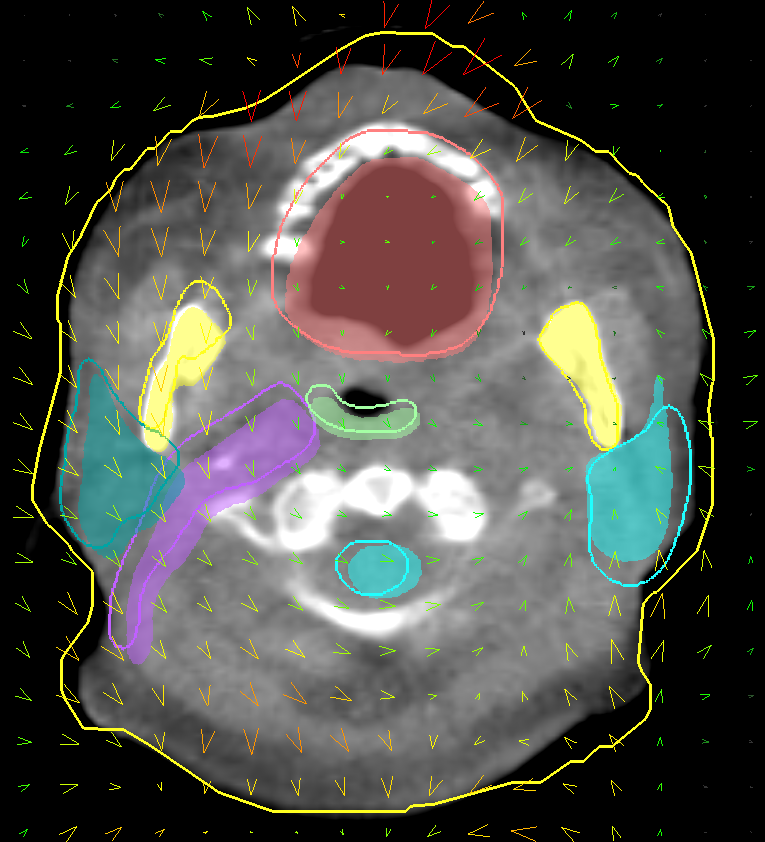
\includegraphics[height=0.6\textheight]{{imgs/patient_deformation}.png}
                \caption{Head and neck patient geometry changes. The arrows represent a vector field.}
            \end{figure}
        \end{column}
    \end{columns}
\end{frame}

% MENTION THAT WE EVALUATE AFTER WARPING THE CONTOURS
% Fix caption
% Add angle to axis labels
\section{The need for adaptive proton therapy}
\begin{frame}[c]{The need for adaptive proton therapy}
    \begin{columns}[c]
        \begin{column}{0.5\textwidth}
            10 head \& neck patients planned \textbf{without CTV margins}, evaluated at 60 weeks:
            \begin{itemize}
                \item Reduced margins $\rightarrow$ sensitive to errors
                \item Coverage deteriorates:
            \end{itemize}
            \vspace*{-0.4cm}
            \begin{figure}[h]
                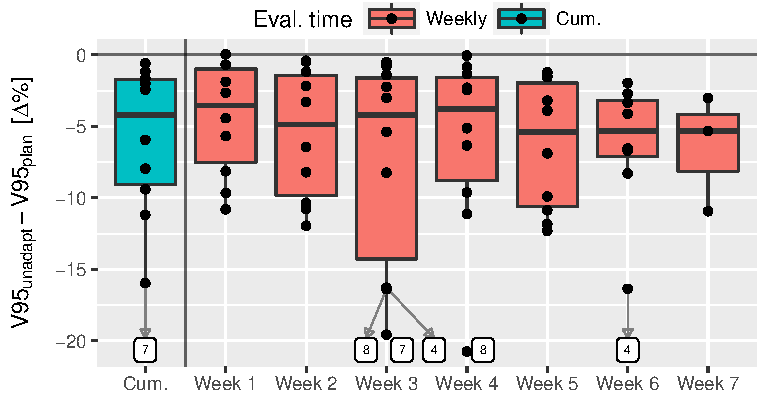
\includegraphics[width=\textwidth]{{imgs/plan_evolution_simple_week.name_V95_diff}.pdf}
                \caption{V95 in CTV decreases}
            \end{figure}
        \end{column}
        \pause
        \begin{column}[c]{0.38\textwidth}
%             \vspace*{-0.5cm}
            \begin{figure}[h]
                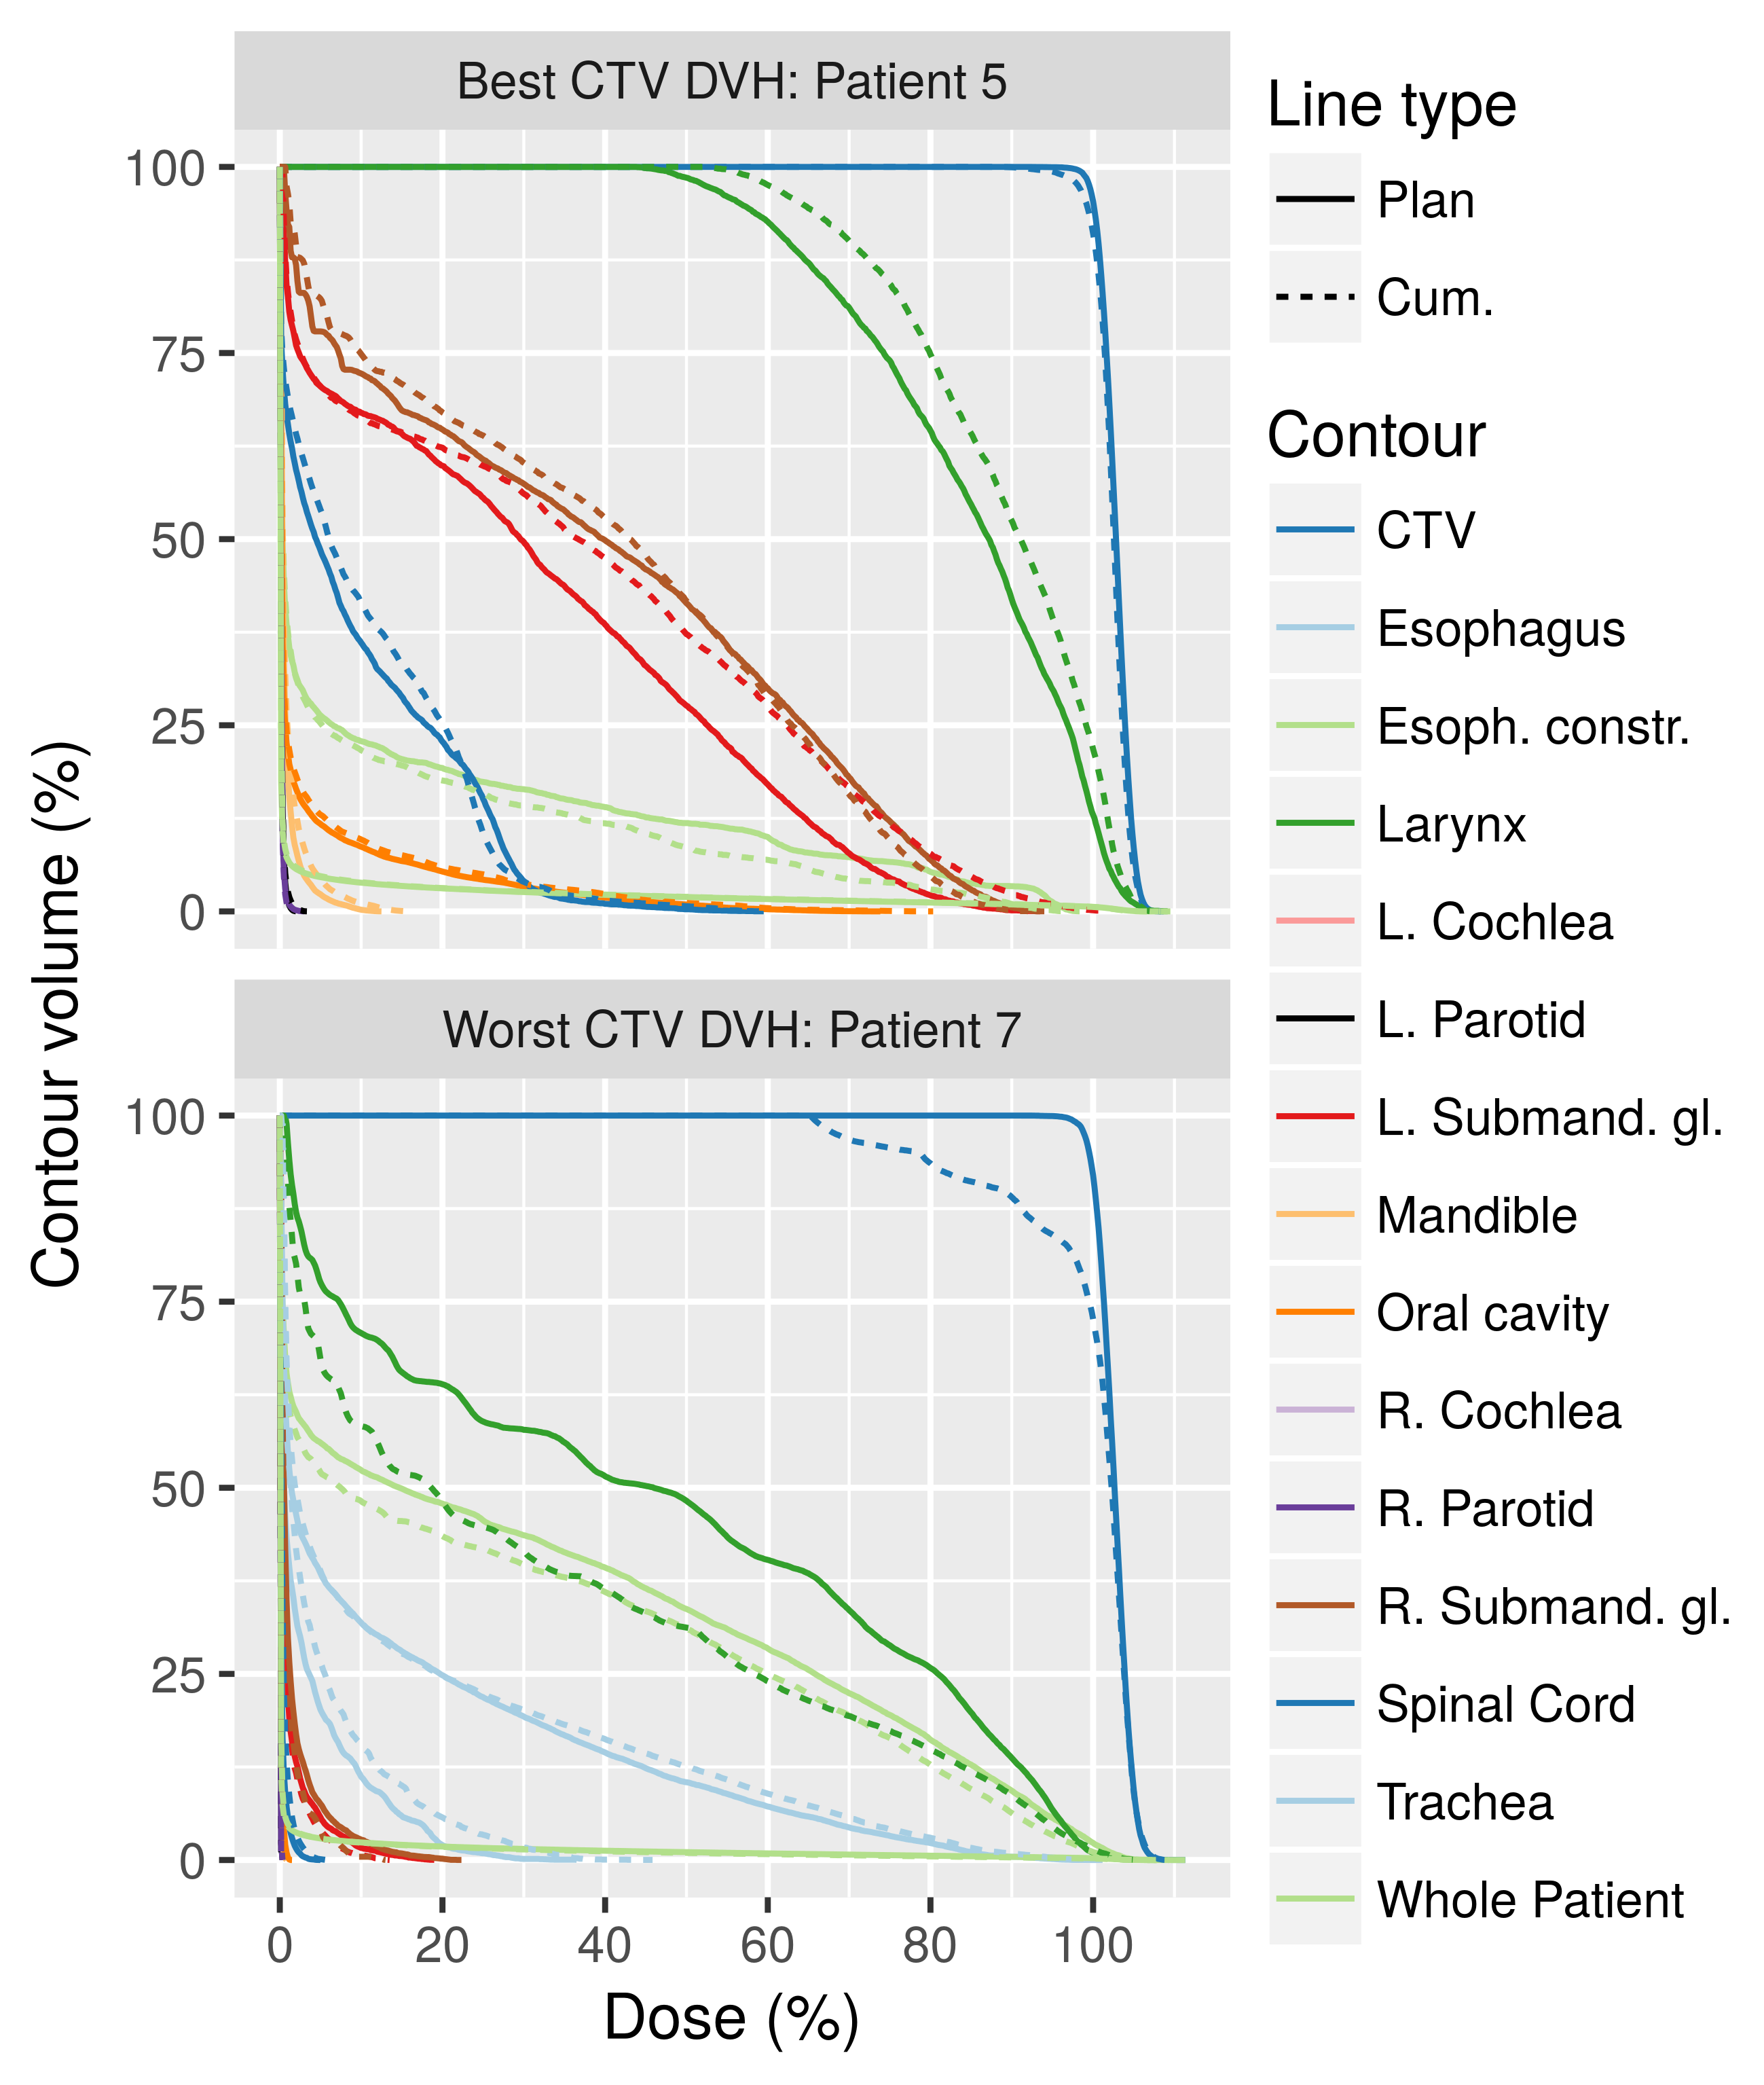
\includegraphics[width=\textwidth]{{imgs/unadapted_cumulative_DVHs}.pdf}
                \caption{DVHs after full treatment}
            \end{figure}
%             \vspace*{-1cm}
%             \begin{figure}[h]
%                 \centering
%                 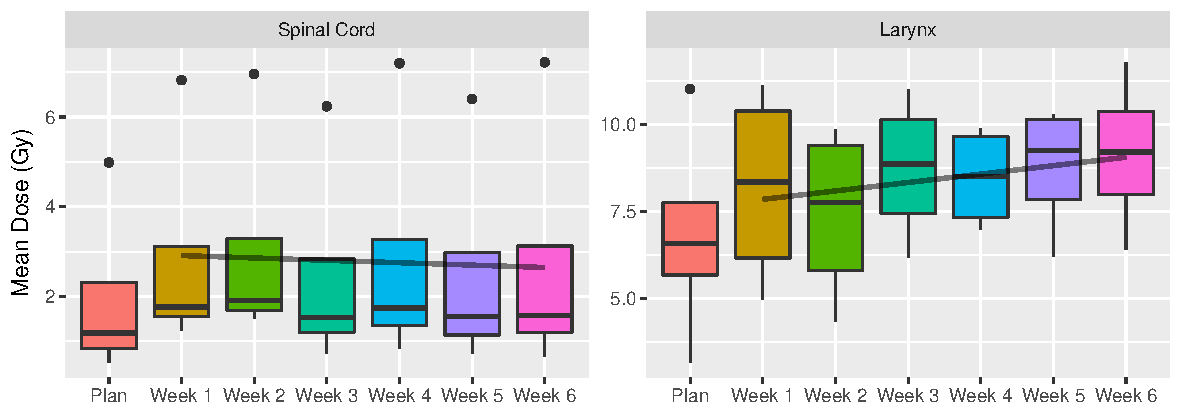
\includegraphics[width=0.9\textwidth]{{imgs/Mean.OARs.reduced.week}.pdf}
%                 \caption{Mean dose increase of spinal cord and larynx}
%             \end{figure}
        \end{column}
    \end{columns}
\end{frame}

\section{Adaptive proton therapy ingredients: the framework}
\begin{frame}[c]{Adaptive proton therapy ingredients: the framework}
    \begin{columns}[c]
        \begin{column}{0.48\textwidth}
            \vspace*{-2mm}
            {\setbeamercolor{block title}{bg=flame, fg=black}
                \begin{block}{Cone Beam CT (CBCT)}
                    \textit{A priori} CT-based scatter correction WEPL error $< 2\%$ in head cases.\\
                    {\begin{flushright}\scriptsize\textit{Park et al., Med Phys. 2015;42(8)}, \textit{Kim et al., Phys Med Bio. 2017;62(1)}\end{flushright}}
                \end{block}}
            {\setbeamercolor{block title}{bg=iceberg, fg=black}
                \begin{block}{Image Registration: Plastimatch}
                    Rigid and deformable (DIR), GPU B-spline\\
                    {\hfill\scriptsize\textit{Shackleford et al., Phys Med Biol. 2010;55(21)}}
                \end{block}}
            {\setbeamercolor{block title}{bg=inchworm, fg=black}
                \begin{block}{Fast GPU MC: gPMC}
                    Accurate calculation engine developed with UT Southwestern.\\
                    {\hfill\scriptsize\textit{Qin et al., Phys Med Biol. 2016;61(20)}}
                \end{block}}
        \end{column}
        \begin{column}{0.5\textwidth}
            \centering
            %question mark has RGBA code ffaf0072
            \includegraphics[width=0.8\textwidth]{{imgs/drawing}.pdf}
        \end{column}
    \end{columns}
\end{frame}

\section{Adaptation method}
\begin{frame}[c]{Adaptation method}
    Consists of 2 steps:
    \begin{enumerate}
        \item {\color{brandeisblue} Geometrical adaptation:} Move individual spots following a deformation vector field and correct energies
        \item {\color{brandeisblue} Weight tuning:} Adjust the weight of the spots, if necessary
    \end{enumerate}
\end{frame}
 


\begin{frame}[c]{Geometrical adaptation}
    \begin{columns}[t]
		\begin{column}{0.55\textwidth}
            Per spot $s_i = (x_0, y_0, E_0)$:
            
            \begin{itemize}
                \item[1:]<2-> \textbf{Raytrace} $s_i$ in CT ($r_i$)
                \item[2:]<3-> \textbf{Probe} VF at $r_i$ coords: $v_i$
                \item[3:]<4-> \textbf{Apply $v_i$ to $r_i$} coords: position where the $r_i$ should be in the CBCT
                \item[4:]<5-> \textbf{Apply $v_i$ to $s$} $\rightarrow $ $s'_i = (x_0 + \Delta v_x, y_0 + \Delta v_y, E_0)_i$
                \item[5:]<6-> \textbf{Raytrace} $s'_i$ in CBCT
                \item[6:]<7-> \textbf{Get} $\Delta E_i$
            \end{itemize}
            \onslide<8>{Spot adaptation: $(\Delta v_x, \Delta v_y, \Delta E)_i$}
		\end{column}
		\begin{column}{0.3\textwidth}
            \vfill
            \includegraphics<1|handout:O>[width=\textwidth]{imgs/adaptation_method_0.pdf}
            \includegraphics<2|handout:O>[width=\textwidth]{imgs/adaptation_method_1.pdf}
            \includegraphics<3|handout:O>[width=\textwidth]{imgs/adaptation_method_2.pdf}
            \includegraphics<4|handout:O>[width=\textwidth]{imgs/adaptation_method_3.pdf}
            \includegraphics<5|handout:O>[width=\textwidth]{imgs/adaptation_method_4.pdf}
            \includegraphics<6|handout:O>[width=\textwidth]{imgs/adaptation_method_5.pdf}
            \includegraphics<7->[width=\textwidth]{imgs/adaptation_method_end.pdf}
		\end{column}
	\end{columns}
\end{frame}

% \begin{frame}[c]{Geometrical adaptation}
%     \begin{columns}[c]
%         \begin{column}{0.45\textwidth}
%             Energy and position layers organization is distorted.
%             \newline
%             
%             \onslide<2>{
%                 Four strategies constraining the geometrical adaptation:
%                 \begin{itemize}
%                     \item {\color{brandeisblue} Free:} No constrains shifts
%                     \item {\color{brandeisblue} Isocenter shift:} Average VF in CTV
%                     \item {\color{brandeisblue} Range shifter:} Average energy shift
%                     \item {\color{brandeisblue} Iso. + range:} Average VF and energy shifts
%                 \end{itemize}
%             }
%         \end{column}
%         \begin{column}{0.55\textwidth}
%             \vspace*{-0.4cm}
%             \begin{figure}[b!]
%                 \centering
%                 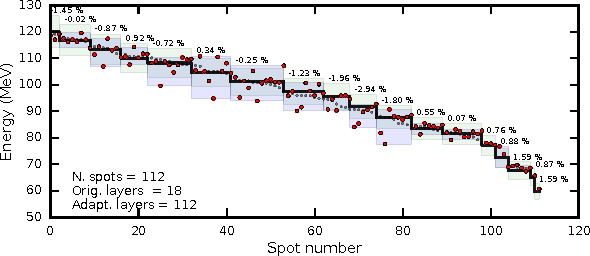
\includegraphics[width=\textwidth]{imgs/plan_energy_layer_destruction.pdf}\\
%                 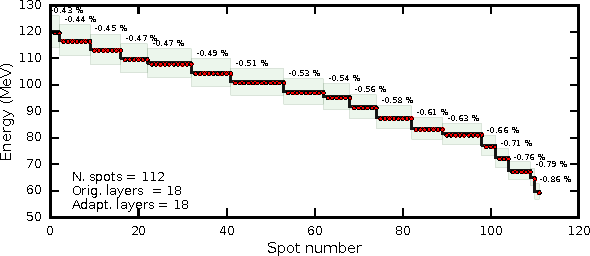
\includegraphics[width=\textwidth]{imgs/plan_energy_layer_conservation.pdf}
%                 \caption{Distortion/conservation of plan energy layers}
%             \end{figure}
%         \end{column}
%     \end{columns}
% \end{frame}

\begin{frame}[c]{Geometrical adaptation}
    Energy and position layers organization is distorted.
    \newline
    
    \onslide<2>{
        Four strategies constraining the geometrical adaptation:
        \begin{itemize}
            \item {\color{brandeisblue} Free:} No constrains shifts
            \item {\color{brandeisblue} Isocenter shift:} Average VF in CTV
            \item {\color{brandeisblue} Range shifter:} Average energy shift
            \item {\color{brandeisblue} Iso. + range:} Average VF and energy shifts
        \end{itemize}
    }
\end{frame}


\begin{frame}[c]{Weight tuning:}
    How to create dose-influence matrices \textbf{fast} with GPU MC (gPMC)?
    \newline
    
    \pause
    
    Observation from initial plans: 8.2\% of the spots deliver 50\% of the protons
    \newline
    
    \pause
	
	Weight tuning steps:
    \begin{enumerate}
    	\item Simulate \textbf{geometrical adaptation} with gPMC
    	\item Score the \textbf{dose per spot} in region of interest
    	\pause
    	\item \textbf{Select set} of spots giving 50\% of the dose (at least 10\% of the total spots)
    	\item Accumulate adapted dose without the set
    	\item Calculate \textbf{remaining dose} for coverage in target
    	\pause
    	\item \textbf{Tune set weights} to fill the remaining dose and spare OARs
    \end{enumerate}
\end{frame}


%IMPT heavily exploits dose irregularities that are not captured in this method
\begin{frame}[c]{Results: all geometrical adaptations (no weight tuning)}
  \pause
    \begin{figure}[b!]
        \centering
        \includegraphics<2|handout:O>[width=\textwidth]{imgs/DVH_points_geometric_nonadapt.pdf}
        \includegraphics<3|handout:O>[width=\textwidth]{imgs/DVH_points_geometric_adapt.pdf}
        \includegraphics<4>[width=\textwidth]{imgs/DVH_points_geometric.pdf}
    \end{figure}
\end{frame}

\begin{frame}[c]{Results: all geometrical adaptations + weight tuning}
    \begin{figure}[b!]
        \centering
        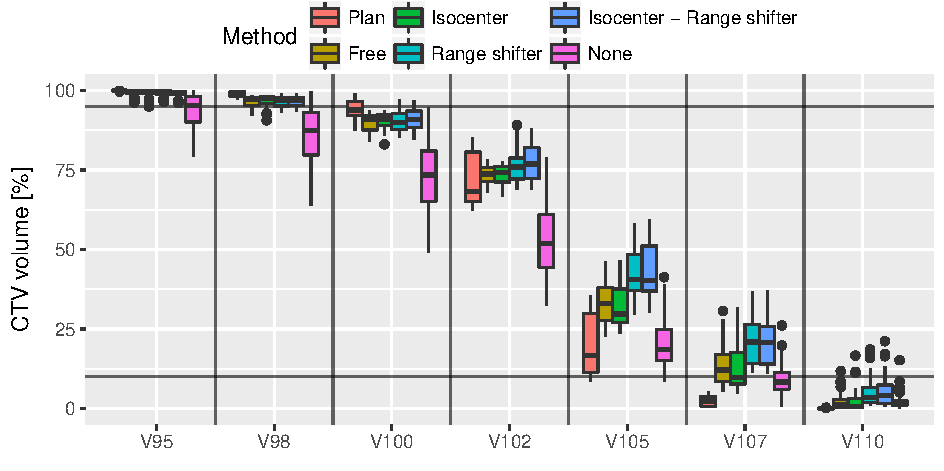
\includegraphics[width=\textwidth]{imgs/DVH_points_weights.pdf}
    \end{figure}
\end{frame}

\begin{frame}[c]{Results with free geometrical adaptation + weight tuning}
    \begin{figure}[b!]
        \centering
        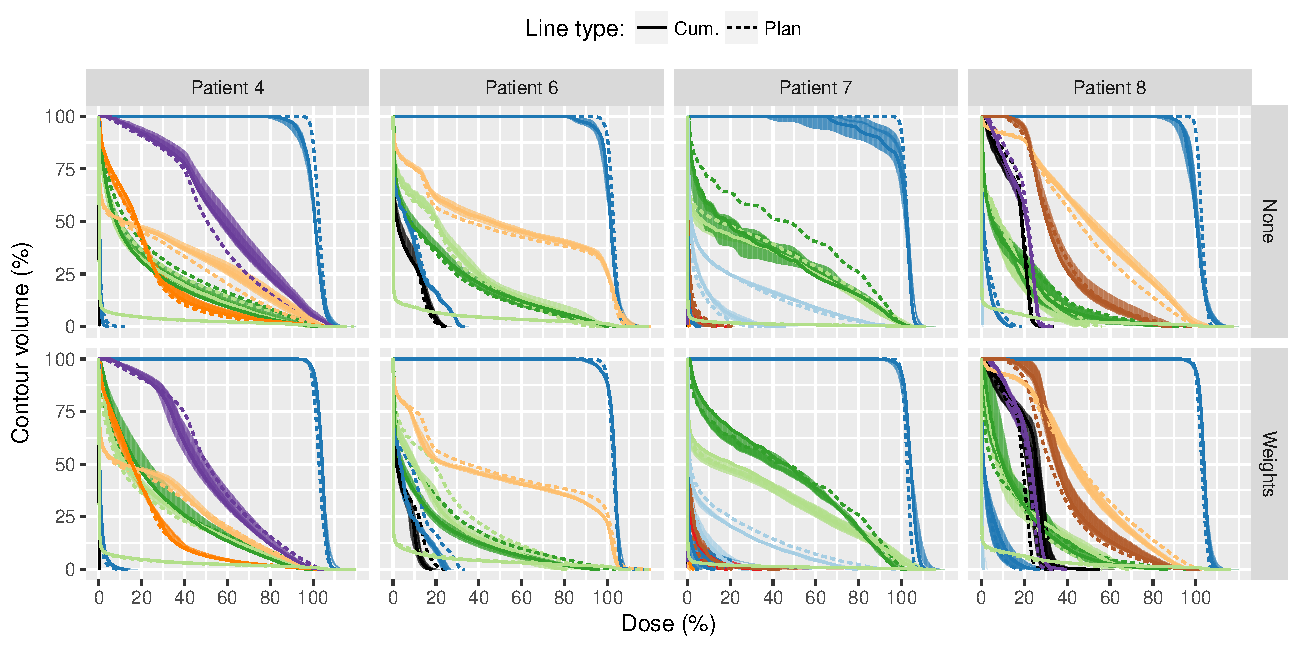
\includegraphics[width=\textwidth]{imgs/adapted_cumulative_DVHs.pdf}
    \end{figure}
\end{frame}


\begin{frame}[c]{Timing and conclusions}
    Timing, timing, timing!!
    \begin{table}[h]
    \scalebox{0.8}{
        \begin{tabular}{l|ccc|c}
            \textit{(seconds)} & Minimum & Average & Maximum & Expected \\
            \hline
            Geometrical adapt. & 11.7  & \textbf{16.9}  & 26.57 & $\sim1-5$ \\
            gPMC validation    & 115.6 & \textbf{261.9} & 419.2 & $\sim30$ \\
            Weight tuning      & 12.0  & \textbf{44.8}  & 198.0 & $\sim5-120$ \\
            \hline
            \textbf{Total}     &   -   & \textbf{322.7} &   -   & $\mathbf{\sim60-120}$ \\
            \hline
        \end{tabular}
        }
        \caption{Current and expected times (s)}
    \end{table}
    \pause

    Conclusions:
    \begin{itemize}
        \item If adaptation is needed, weight tuning is generally necessary
        \item Tuning the \textbf{weight of a subset of spots} might be enough
        \item The algorithm has the potential to \textbf{be applicable online, pending hardware and parallelization}
        \item The algorithm might \textbf{allow further margin reduction}
    \end{itemize}
\end{frame}

\begin{frame}[plain]
    \centering
    \begin{figure}[h]
%         
\includegraphics[width=0.7\textwidth]{imgs/thanks.png}
        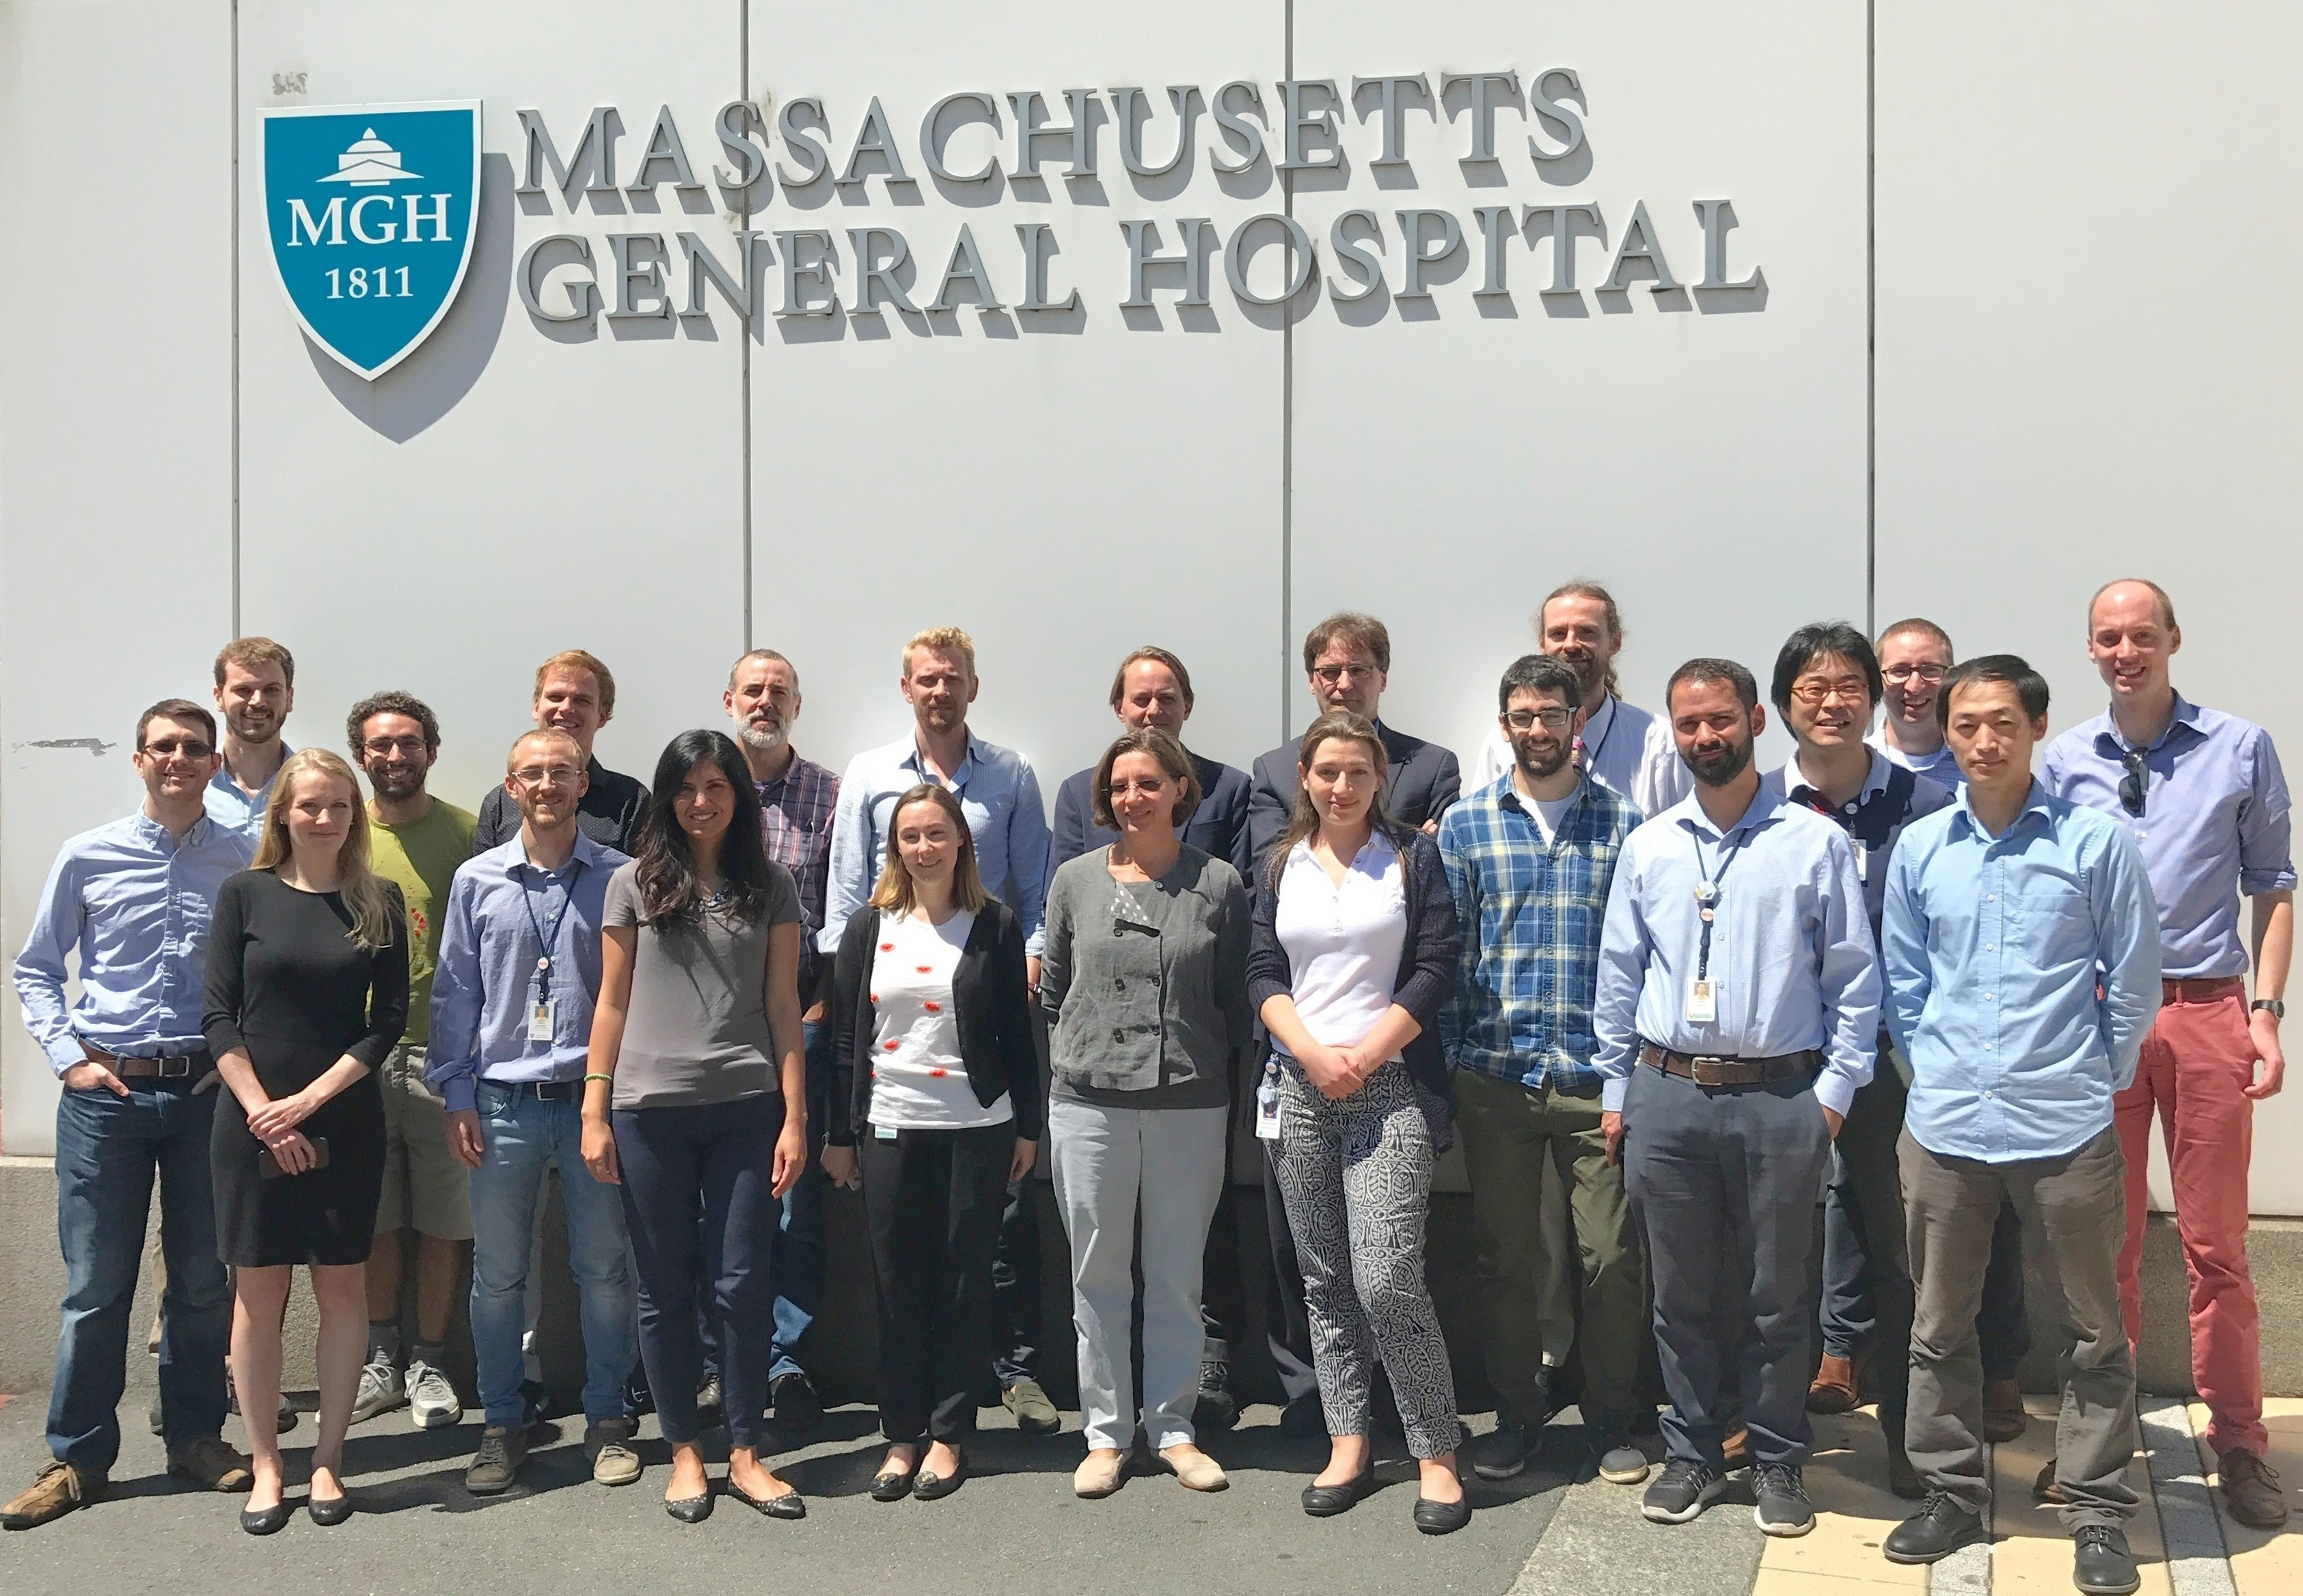
\includegraphics[height=0.9\textheight]{imgs/group.JPG}\\
        Visit \url{https://gray.mgh.harvard.edu/}!
    \end{figure}
\end{frame}

\end{document}
